% !TeX root = ../libro.tex
% !TeX encoding = utf8



\setchapterpreamble[c][0.75\linewidth]{%
	\sffamily
  
      El objetivo de este capítulo es motivar e introducir al lector en el problema, para ello se abordará el asunto desde un aspecto descriptivo. Primeramente se realizará una descripción del problema, exponiendo la necesidad e importancia de enfrentar este tipo de problemas. Después, se presentará una sección que explica los electrocardiogramas para que de este modo el lector adquiera un mayor conocimiento del tema y le resulten familiares en lo que sigue. Posteriormente se hablará de la base de datos usada así como del principal inconveniente que presenta. Finalmente se incluirá un estado del arte en el que el lector podrá ponerse en contexto en cuanto al avance de este campo.

	\par\bigskip
}

\chapter{Descripción del problema}\label{ch:descripcion_problema}

\section{Descripción del problema}

    La fibrilación auricular es un ritmo cardíaco irregular y a menudo muy rápido (arritmia) que puede provocar coágulos de sangre en el corazón. Tener una fibrilación auricular incrementa la probabilidad de sufrir un accidente cerebrovascular, insuficiencia cardíaca y otras muchas complicaciones relacionadas con el corazón. Es una enfermedad que afecta a millones de personas en todo mundo y no entiende de género y edades. Sí es cierto que es más frecuente en personas de edad avanzada, pero en los últimos años se han incorporado muchos casos en jóvenes y adultos. Por este motivo, es de vital importancia poner las tecnologías más avanzadas en este área con objeto de salvar todas las vidas que se puedan y mejorar la calidad de las mismas. \\
    
    Se nos presenta un problema de clasificación de señales obtenidas por electrocardiogramas (ECG). El principal objetivo es discernir entre ritmos normales, es decir, aquellos ritmos propios de una persona sin patologías cardíacas y entre fibrilaciones auriculares (FA). No obstante, existen otras enfermedades parecidas a la fibrilación auricular, por este motivo, también es de vital importancia discernir entre estas otras enfermedades y la FA, ya que los tratamientos a seguir no van a ser iguales en caso de tener un tipo de enfermedad u otra. \\
    
    Para enfrentarnos al problema se ha recurrido a uno de los paradigmas dentro la inteligencia artificial que abordan este asunto de forma novedosa, el aprendizaje profundo. Este paradigma presenta una gran ventaja frente a los tradicionales, y es la ausencia a priori de conocimiento experto del tema, haciendo que cualquier persona pueda emprender el desarrollo de un problema de este tipo sin la necesidad de ser un experto en el tema. \\ 
    


\section{Electrocardiogramas}
    
    
    Un electrocardiograma, abreviado como ECG es un procedimiento médico indoloro, no invasivo y simple que registra la actividad eléctrica del corazón. Los latidos del corazón son posibles gracias a una pequeña señal eléctrica que circula por este órgano y es la responsable de guiar las contracciones y expansiones de las cavidades que lo forman. Un ECG muestra si su corazón está latiendo a un ritmo y con una fuerza normal, suponiendo un problema para la salud en caso contrario. Dicho en otras palabras, el ECG representa de manera visual la actividad eléctrica del corazón en función del tiempo, obtenida desde la superficie corporal del pecho. \\
    
    
    El ECG se usa para encontrar y vigilar varias enfermedades del corazón tales como obstrucción de arterias, insuficiencia cardíaca, arritmias (latidos cardíacos irregulares), ataques del corazón, obstrucción de arterias entre otras. \\
    
    Las partes de un ECG las podemos encontrar en la imagen \ref{fig:ECG}. Un ECG corriente que registra un latido cardíaco normal consta de una onda P, un complejo QRS, y una onda T. Generalmente, la onda U suele ser invisible. Estos fenómenos eléctricos no han de confundirse con los fenómenos mecánicos de contracción y relajación de las cavidades del corazón. La contracción del ventrículo, a lo cual nos referiremos a partir de ahora como sístole mecánica, comienza justo después del inicio del complejo QRS y termina justo antes del finalizar la onda T. La diástole, que es cuando la ventrículo se relaja y se rellena comienza justo después de que acabe la sístole correspondiente a la contracción de las aurículas, justo después de comenzar la onda P. \\
    
    La onda P es la señal que corresponde a la despolarización auricular. Esta onda es la responsable de provocar la contracción de las aurículas. El compejo QRS corresponde a la señal de despolarización ventricular e indica el inicio de la contracción de la ventrícula. Este complejo está formado por tres ondas, la Q, la R y la S. La onda Q es una onda negativa y representa una pequeña desviación previa a la sístole ventricular, la onda R es la primera deflexión positiva del complejo QRS y es la de mayor tamaño, es la responsable de la contracción de los ventrículos y finalmente, la onda S, es cualquier onda negativa que siga a la onda R. La onda T representa la relajación por parte de los ventrículos. Estas ondas aparecen una vez por cada pulso del corazón y cuando nos tomamos el pulso contamos el número de veces que se repite la onda R por intervalo de tiempo. Cualquier irregularidad en algunas de estas ondas puede dar lugar a enfermedades coronarias. \\
    
    \begin{figure}[H]
        \centering
        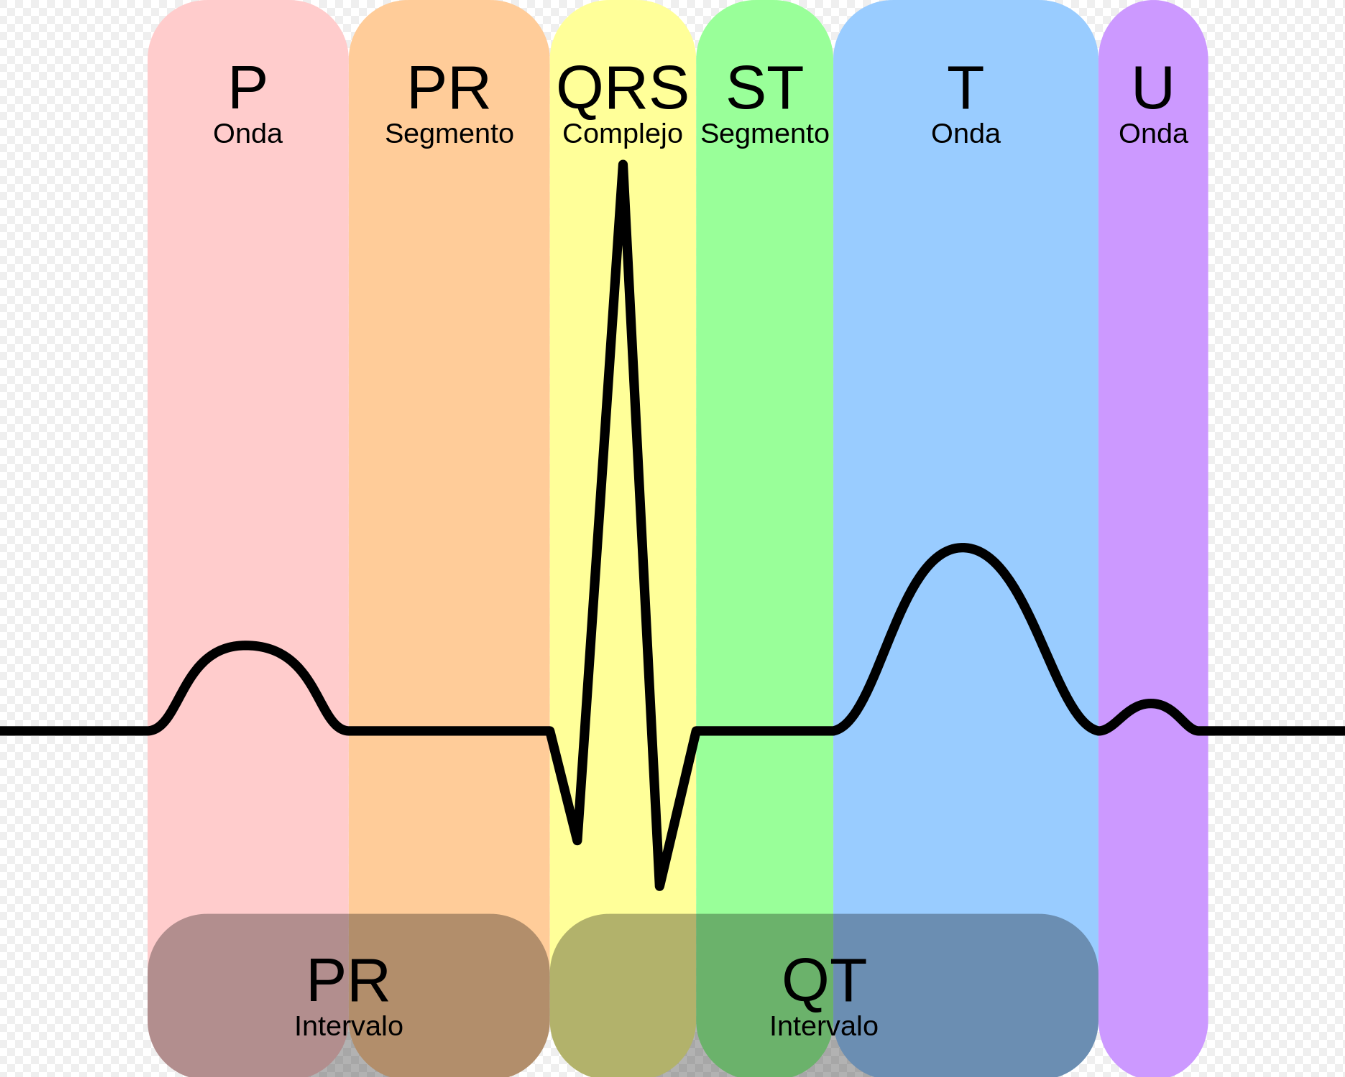
\includegraphics[height=5cm, width = 7cm]{img/ECG_2.png}
        \caption{Representación de un ECG normal distinguiendo por intervalos las distintas partes.\href{https://upload.wikimedia.org/wikipedia/commons/thumb/e/e8/EKG_Complex_es.svg/1280px-EKG_Complex_es.svg.png}{Fuente}}
        \label{fig:ECG}
    \end{figure}
    
    
    
    

\section{Base de Datos Experimental}

    Vamos a trabajar con una base de datos propuesta para una competición en el año 2017 por la plataforma \textit{PhysioNet/CinC} llamada \textit{AF Classification from a Short Single Lead ECG Recording: The PhysioNet/Computing in Cardiology Challenge 2017} y disponible a través de este a través de este \href{https://physionet.org/content/challenge-2017/1.0.0/}{enlace}. El objetivo de esta competición es fomentar el desarrollo de algoritmos que permitan clasificar, a partir de un único registro de derivación de ECG corto (entre 30 y 60 segundos), si el registro muestra un ritmo sinusal normal, una fibración auricular (FA), un ritmo alternativo o es demasiado ruidoso como para ser clasificado. \\
    
    Se define la FA como una \textit{taquiarritmia caracterizada por una activación auricular predominantemente descoordinada con el consiguiente deterioro de la función mecánica auricular}. La AF es la arritmia cardiaca sostenida más frecuente, que se presenta en el 1-2\% de la población general y viene asociada a una alta mortandad y morbilidad por la asociación de riesgo de muerte, ictus, hospitalización, insuficiencia cardiaca, etc. Aproximadamente más de 12 millones de personas de Europa y América padecen FA y su prevalencia se estima que será del triple de aquí a 30-50 años. Otro dato a tener en cuenta, es que la incidencia de la FA aumenta con la edad, desde menos del 0,5\% a los 40-50 años, hasta el 5-15\% en personas de 80 años. \\
    

    La detección de la FA es bastante compleja, ya que puede ser episódica. Los detectores de FA pueden considerarse pertenecientes a dos categorías: métodos basados en el análisis de la actividad auricular o en el análisis de la respuesta ventricular. Los primeros se basan en el análisis de la ausencia de ondas $P$ o la presencia de ondas $f$ fibrilatorias en el intervalo $TQ$. Estos métodos son muy sensibles a la contaminación, pero presentan la ventaja de ser bastante precisos si las señales están poco contaminadas y tienen una alta resolución. El segundo se basa en la predictibilidad del tiempo entre latidos (intervalos RR) de los complejos QRS en el ECG. Los intervalos RR se derivan de la característica de gran amplitud más obvia del ECG, el pico R, cuya detección puede ser mucho más resistente al ruido y por ello, se suele usar para detección automática de FA en tiempo real. \\

        Los estudios anteriores relativos a la clasificación de la FA suelen tener una aplicabilidad limitada ya que
        \begin{itemize}
            \item Solo se realizó la clasificación de los ritmos normales y de la FA
            \item El buen rendimiento se demostró en datos cuidadosamente seleccionados y a menudo limpios
            \item No se utilizó un conjunto de datos de prueba fuera de la muestra
            \item Sólo se utilizó un pequeño número de pacientes
        \end{itemize}

    
        
    Es bastante complejo detectar la FA de manera suficientemente fiable a partir de una sola derivación corta del ECG. Además, la amplia variedad de ritmos existentes tampoco facilita nada las cosas. En particular, hay muchos ritmos que no son FA y presentan intervalos RR irregulares que pueden ser similares a la FA. En este desafío, tratamos todos los ritmos anormales no relacionados con la FA como una sola clase y clasificamos los ritmos como: \\
        
        \begin{itemize}
            \item Ritmo sinusal normal (Paciente Sano)
            \item FA (Fibrilación auricular)
            \item Otro Ritmo
            \item Electrocardiogramas ruidosos
        \end{itemize}
        
        \begin{figure}[H]
            \centering
            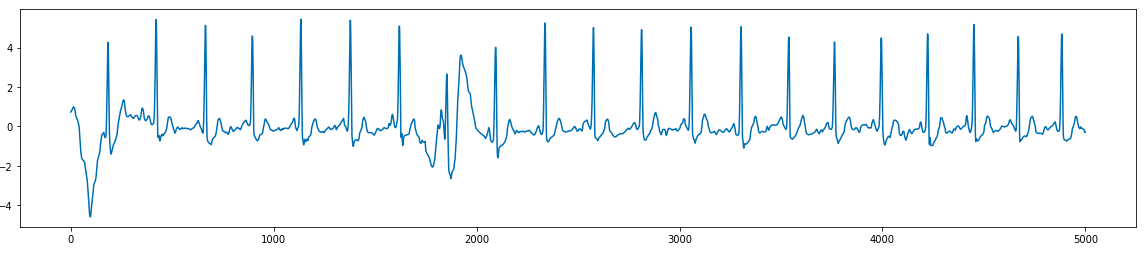
\includegraphics[width=15cm,height=4cm]{Normal.png}
            \caption{Ritmo Sinusal Normal}
            \label{fig:normal}
        \end{figure}
        
        
        \begin{figure}[H]
            \centering
            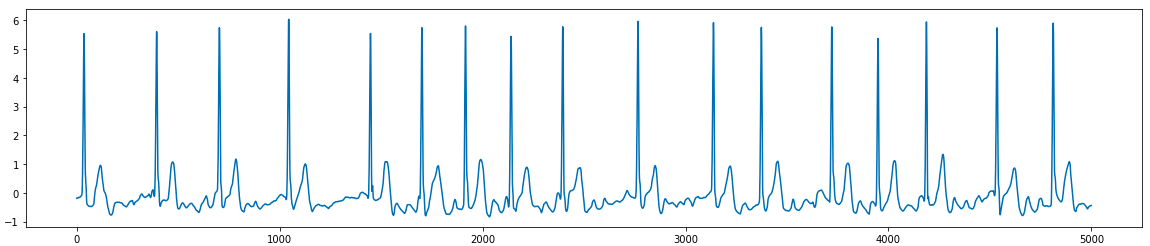
\includegraphics[width=15cm,height=4cm]{FA.png}
            \caption{Fibrilación Auricular}
            \label{fig:af}
        \end{figure}
        
        \begin{figure}[H]
            \centering
            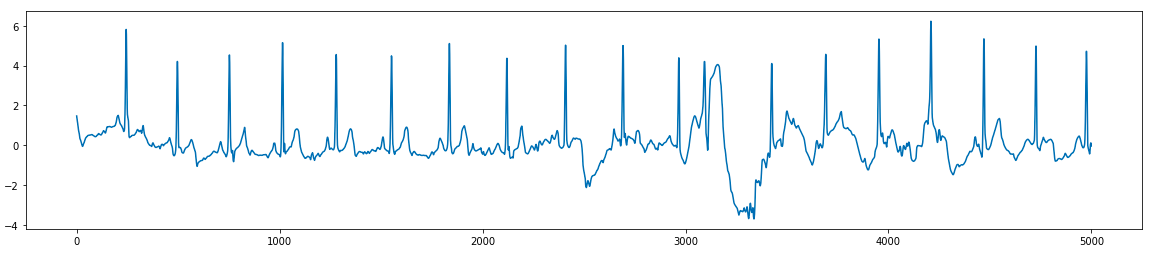
\includegraphics[width=15cm,height=4cm]{Other.png}
            \caption{Otro ritmo}
            \label{fig:other}
        \end{figure}
        
        \begin{figure}[H]
            \centering
            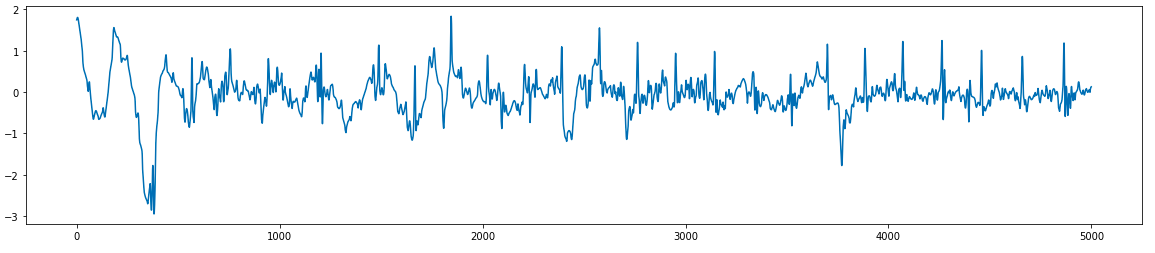
\includegraphics[width=15cm,height=4cm]{noise.png}
            \caption{Electrocardiograma Ruidoso}
            \label{fig:noise}
        \end{figure}
        

        En las figuras \ref{fig:normal},\ref{fig:af},\ref{fig:other} y \ref{fig:noise} mostramos un ejemplo de como sería cada señal. Visualmente puede distinguirse presencia de un ruido en la señal correspondiente a la figura \ref{fig:noise} y \ref{fig:other}, pero nada que ver con \ref{fig:noise} la cual tiene ruido en cantidades excesivas. \\
        
        
        \begin{table}[htbp]
        \caption{Datos del conjunto de entrenamiento}
        \begin{center}
        \begin{tabular}{|l|r|r|r|r|r|r|}
        \hline
        \textbf{Tipo} & \multicolumn{1}{l|}{\textbf{Cantidad}} & \multicolumn{1}{l|}{\textbf{Media}} & \multicolumn{1}{l|}{\textbf{SD}} & \multicolumn{1}{l|}{\textbf{Max}} & \multicolumn{1}{l|}{\textbf{Mediana}} & \multicolumn{1}{l|}{\textbf{Min}} \\ \hline
        \textbf{Normal} & 5154 & 31,9 & 10 & 61 & 30 & 9 \\ \hline
        \textbf{AF} & 771 & 31,6 & 12,5 & 60 & 30 & 10 \\ \hline
        \textbf{Otro Ritmo} & 2557 & 34,1 & 11,8 & 60,9 & 30 & 9,1 \\ \hline
        \textbf{Ruido} & 46 & 27,1 & 9 & 60 & 30 & 10,2 \\ \hline
        \textbf{Total} & 8528 & 32,5 & 10,9 & 61 & 30 & 9 \\ \hline
        \end{tabular}
        \end{center}
        \label{table:BD}
        \end{table}
        
        De la tabla \ref{table:BD} podemos observar el notorio desbalanceo de clases en el conjunto de datos. La clase mayoritaria correspondiente a los ritmos normales presentan casi el $60\%$ de los datos y la minoritaria, un poco más del $3\%$. Esto viene a indicar que el proceso de aprendizaje va a ser una tarea complicada, pues los modelos se van a especializar en clasificar la clase mayoritaria dejando de lado la minoritaria. \\
        
        Para tratar este desbalanceo se pueden emplear infinidad de técnicas, aunque en el contexto de la competición no son todas válidas. Por ejemplo, se podría pensar en eliminar la clase minoritaria por tener una representación ínfima del conjunto, sin embargo, las reglas establecen que eso no debe hacerse, pues a fin de cuentas estaremos sesgando los resultados y bajo el supuesto de que el modelo se implemente en la práctica, resultará en algo muy poco fiable y propenso a fallos. Por otra parte existen técnicas específicas para tratar el desbalanceo de ECG. Algunos investigadores como Sanabila et al. \cite{sanabila2016generative} utilizaron el método de sobremuestreo generado (GenOMe) para resolver el problema de las arritmias desequilibradas, que generaba nuevos puntos de datos con distribuciones específicas (beta, gamma y gaussiana) como restricciones. Y otros como Rajesh y Dhuli \cite{rajesh2018classification} emplearon tres técnicas de preprocesamiento a nivel de datos en un conjunto de características extraídas para equilibrar la distribución de los latidos del ECG. Estas técnicas fueron el sobremuestreo y submuestreo aleatorio (ROU), la técnica de sobremuestreo minoritario sintético con submuestreo aleatorio (SMOTE + RU) y el equilibrio basado en la distribución DBB. Sin embargo, nosotros no emplearemos técnicas tan sofisticadas para tratar ese problema. Las técnicas empleadas entran en la parte del preprocesado de datos que se comentará en el capítulo siguiente. \\
        
    

\section{Estado del Arte}

El electrocardiograma (ECG) es la herramienta de diagnóstico más común con un bajo coste utilizada para detectar las señales eléctricas del corazón. Las señales cardíacas anormales se conocen como arritmia y puede ser peligrosa o, en la mayoría de los casos, puede causar incluso la muerte. La arritmia puede ser de distintos tipos, y puede ser detectada por una prueba de ECG. El cribado automatizado de la clasificación de la arritmia mediante los latidos del ECG se desarrolla desde hace años. Los sistemas automatizados que pueden adaptarse como herramienta para la clasificación de arritmias desempeñan un papel vital no solo para los pacientes, sino también para los médicos. Las técnicas de clasificación de arritmias automatizadas basadas en el aprendizaje profundo se han desarrollado con resultados de alta precisión, pero aún no han sido adoptadas por los profesionales de la salud como un enfoque generalizado porque en los estudios recientes los autores utilizaron datos de series temporales, que no son adaptables en diferentes entornos de aplicación.  \\
    
    
    Según los datos facilitados por la \href{http://www.who.int/mediacentre/factsheets/fs317/en/.}{Organización Mundial de la Salud (OMS)} en 2020 murieron entorno a 25 millones de personas debido a este tipo de patologías. La prueba del electrocardiograma (ECG) se utiliza como herramienta de diagnóstico en los centros sanitarios pero son los profesionales sanitarios los que diagnostican manualmente el estado del corazón del paciente interpretando la imagen del ECG. Gracias al avance de la tecnología, se han desarrollado varias herramientas de diagnóstico automático para la clasificación y detección de arritmias con el fin de asistir a los médicos.\\
    
    De este modo, se empezó a investigar de forma crítica los latidos del corazón y herramientas de detección y clasificación. Desde su comienzo hasta hoy, podemos distinguir dos tipos de metodologías empleadas. Por un lado tenemos a la más tradicional. Esta vertiente se caracteriza por la necesidad de que el investigador tenga un conocimiento a priori sobre el tema, pues es él mismo quien decide de manera manual qué características extraer de las señales y cómo hacerlo. Poco a poco fue entrando en juego técnicas de aprendizaje profundo las cuales son capaces de extraer características por cuenta propia sin necesidad de conocimiento a priori por parte del investigador. Destacamos el trabajo de Khan et al. \cite{khan2021cardiac} que proporciona una introducción muy completa de los estudios relacionados en el dominio del problema y propone una técnica basada en redes neuronales profundas, para la clasificación de tres tipos de latidos de arritmia. \\
    
    Las últimas tendencias que se están usando son las arquitecturas de aprendizaje profundo, tras el estudio de numerosos artículos publicados sobre clasificación de arritmias (\cite{ohshuli,GaoJunLi,chenchen, zhang2020ecg,lynn2019deep,yao2020multi,gao2021end,tan2018application,sajjad2020novel,zheng2020automatic,wang2019photovoltaic,kim2019predicting,kim2020ensemble,geng2020epileptic,fu2019hybrid,huang2020classification,lih2020comprehensive,wei2019early,kong2019convolution,yildirim2019new,cai2020accurate,hou2019lstm}) destaca que los métodos más comúnmente usados son las redes neuronales recurrentes (RNN), LSTM, Autoencoder, CNN,  DNN y redes de creencias profundas. De hecho, en la imagen \ref{fig:trend state of art} podemos apreciar la tendencia actual en el uso de técnicas empleadas para este problema. Observamos que por antonomasia la más empleada es la CNN, pues la que mejor se encarga de extraer las características. Le sigue las redes neuronales profundas junto con las redes neuronales recurrentes y las LSTM. El autoencoder es otra técnica muy usada la cual realiza una reducción de la dimensionalidad, y trata de generar una clase similar a su entrada original. En numerosos estudios de investigación se aplicaron variaciones de la arquitectura de una red neuronal profunda con LSTM y autoencoder. En particular en el estudio \cite{hou2019lstm}, el autor propuso una arquitectura de LSTM con autoencoder combinada con una máquina de soporte vectorial (SVM) para la clasificación de arritmias en ECG. La red basada en LSTM-AE se dedicaba a aprender las características de las señales del ECG mediante un modelo codificador que extrae información de alto nivel de las señales a través de la red LSTM y un modelo decodificador que reconstruye las señales a partir de las características de alto nivel extraídas. La SVM se usaba para clasificar las señales a partir de las características aprendidas. Los resultados del estudio demostraron que la técnica propuesta aprendía mejores características que el método tradicional y sin ningún conocimiento previo, presentando así un buen potencial. Otros estudios como \cite{yildirim2019new} combinaban CNN, LSTM y autoencoder produciendo de igual manera, resultados bastante satisfactorios.\\
    
    La CNN es considera una herramienta de vanguardia para la clasificación de arritmias, y se ha estudiado con diversas variaciones, como la unidimensional, la bidimensional o la combinación de ambas \cite{xiao2020heart,noman2019short}. Según \cite{xiao2020heart}, una nueva técnica de clasificación de arritmias consta de tres fases: preprocesamiento, arquitectura CNN unidimensional, y votación por mayoría para predecir el resultado final. Por otra parte, en \cite{noman2019short} se propuso un marco basado en una CNN unidimensional para el aprendizaje directo de características a partir de los latidos de arritmia sin procesar y una CNN bidimensional, que toma mapas de características de tiempo-frecuencia bidimensionales. \\ 
    
    A día de hoy, se ha desarrollado un sistema automatizado que predice resultados de alta precisión para la detección de arritmias, en embargo aún no puede ser adoptado por los profesionales del sector de la salud. Las principales preocupaciones que afectan al éxito de los sistemas de detección de arritmias desarrollados son (i) la selección manual de características, (ii) las técnicas utilizadas para la extracción de características, (iii) el algoritmo utilizado para la clasificación, y (iv) el uso de datos desequilibrados para la clasificación siendo este último el más importante. \\ 
    
    
    Comentar que todos los estudios consultados han usado bases de datos públicas y totalmente disponibles para la comunidad investigadora. El principal inconveniente que presentan es la escasa cantidad de instancias que presentan algunas. En la imagen \ref{fig:db ecg} observamos las distintas bases de datos empleadas. Comentar que la mayoría no son específicas a su contexto clínico. Falta la descripción de la población de pacientes en la que se obtuvieron estos ECG, algo de vital importancia para poder interpretar la metodología y la utilidad clínica en su contexto. 
    
    \begin{figure}[htpb]
        \centering
        \includegraphics[scale=0.4]{img/state of art image.png}
        \caption{Tendencia actual de las técnicas usadas para clasificación de arritmias.Imagen obtenida de \cite{khan2021arrhythmia}}
        \label{fig:trend state of art}
    \end{figure}
    
    \begin{figure}
        \centering
        \includegraphics[width=\textwidth,height=\textheight,keepaspectratio]{img/database table.png}
        \caption{Base de datos de ECG dedicadas a clasificación de arritmias. Imagen obtenida de \cite{khan2021arrhythmia}}
        \label{fig:db ecg}
    \end{figure}
    
    
    

    
\endinput